\newcommand{\hyperopt}{\texttt{Hyperopt}}

\section{Hyper-optimization}
\label{sec:hyper-opt}

We want to address the problem of finding the minimum of an {\em unknown}\ function $f$,
\begin{equation}
    \label{eq:FDef}
    f: \Omega \to \mathbb{R}\, ,
\end{equation} 
where $\Omega$ is a compact subset of $\Rd$. Although $f$ is unknown, we assume
that we can perform {\em noisy}\ estimates of $y=f(x)$ for given values of $x$,
such that
\begin{equation}
    \label{eq:UnbiasedEval}
    \Ebb\left[y|f(x)\right] = f(x)\, ,
\end{equation}
where the average here is over the fluctuations of $y$. Our knowledge of the function $f$ is encoded in the probability distribution function of $f(x)$ for each value of $x$. At the beginning of the process we need to choose a prior distribution for these values. The prior distribution is then updated according to the value of noisy measurements of $f$ at given values of $x$.  

Bayesian Optimization is an algorithm that performs a {\em sequential} search by
selecting at every step a position $x$ in $\Omega$ according to some acquisition
function, and computing the corresponding value of $y$. After $\nopt$ iterations
the algorithm yields its current best estimate of the position of the minimum.
The procedure is summarised in Fig.~\ref{fig:BOpt}, taken from
Ref.~\cite{shahriari2015taking}.

\begin{figure}[ht!]
    \label{fig:BOpt}
    \centering
    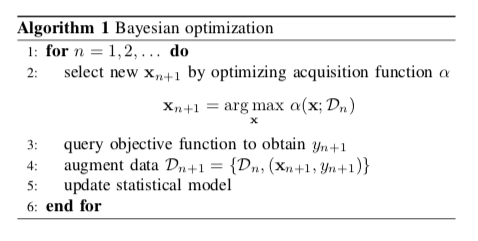
\includegraphics[scale=0.5]{BayesianOptAlg.png}
    \caption{\small Summary of the Bayesian Optimization procedure.}
\end{figure}

\paragraph[]{Summary} The important ingredients in BO are the following. 
%
\begin{enumerate}
    \item[$\bullet$] Choice of the space of parameters, which we denoted $\Omega$ above.  
    \item[$\bullet$] Choice of the loss function $f$, and methodology to evaluate it. 
    \item[$\bullet$] Update of the prior distribution for $f(x)$.
    \item[$\bullet$] Choice of the acquisition function $\alpha$.
    \item[$\bullet$] Choice of the value of $x$ for a new measurement, given the acquisition function.   
\end{enumerate}
%
We need to specify each of these steps in our procedure. 


\subsection{Parametric Models}
\label{sec:BaysParMod}

There are interesting results on parametric models, which are useful to
understand the idea behind BO. In parametric models the function $f$ is
specified by a set of parameters $w$. The current knowledge of $f$ is then
encoded in the probability distribution of these parameters. 

\paragraph[]{Explicit Examples}

\subsection{Non-parametric Models}
\label{sec:BaysNonParMod}

A Gaussian Process $\mathrm{GP}(\mu, k)$ is fully characterised by its mean
function $\mu: \Omega\to \Rbb$, and its kernel function $k: \Omega \times \Omega
\to \Rbb$. We are going to use a Gaussian Process to define the prior for the
unknown function $f$. For a collection of points $\{x_i, i=1,\ldots,n\}$, we
have a set of values $\{f_i=f(x_i), i=1,\ldots,n\}$ and their noisy estimates
$\{y_i, i=1\ldots, n\}$. Remember that $x_i\in\Omega$ is a $d$-dimensional real
vector for every value of $i$. Their respective distributions will be: 
\begin{align}
    \label{eq:GPone}
    \mathbf{f}|\mathbf{x} &\sim 
        \mathcal{N}\left(\mathbf{m},\mathbf{K}\right)\, ,\\
    \mathbf{y}|\mathbf{f},\sigma &\sim 
        \mathcal{N}\left(\mathbf{f},\sigma^2\right)\, ,
\end{align}
where $m_i=\mu(x_i)$ and $K_{ij}=k(x_i,x_j)$. In Eq.~\eqref{eq:GPone} we denote
by boldface fonts vectors and matrices in the $n$-dimensional space of
measurements that have been performed. 

After $n$ observations $\mathcal{D}_n=\left\{\left(x_i,y_i\right)\right\}$, the random variable $f(x)$ is Gaussianly distributed, 
\begin{equation}
    \label{eq:PostGaussF}
    f(x)\sim \mathcal{N}\left(\mu_n(x),\sigma_n(x)\right)\, ,
\end{equation}
with
\begin{align}
    \label{eq:PostParams}
    \mu(x) &= \mu(x) + \mathbf{k}(x)^T \left(\mathbf{K} + \sigma^2 \mathbf{I}\right)^{-1} \left(\mathbf{y}-\mathbf{m}\right)\, , \\
    \sigma(x)^2 &= k(x,x) - \mathbf{k}(x)^T \left(\mathbf{K} + \sigma^2 \mathbf{I}\right)^{-1} \mathbf{k}(\mathbf{x})\, .
\end{align}
This posterior distribution encodes our knowledge of the function $f$ at a
generic point $x\in\Omega$. It is then used to select the next point in the
search. 

\subsection{Acquisition Function}
\label{sec:AcqFun}

In BO the choice of the next point $x$ where the function $f$ is going to be
evaluated plays a crucial role. Choosing a random point would be extremely
inefficient, especially if the dimensionality of the space is increased. 

An informed choice of the point $x$ can be made from the knowledge of the
posterior distribution of $f$, and a utility function $U(x,v)$, where $v=f(x)$.
The utility function describes in some sense how much information is provided by
a measurement at $x$. Since $f$ is unknow, we can marginalise with respect to
$v$ using the probability distribution discussed above and define the {\em
expected utility} of a query point:
\begin{equation}
    \label{eq:ExpUtilDef}
    \alpha(x,\mathcal{D}_n) = \Ebb_{v|\mathcal{D}_n}\left[U\left(x,v\right)\right]\, .
\end{equation} 

\paragraph[]{Improvement-based policies}

The acquisition function favours points that are likely to exceed some target value $\tau$; this strategy is called {\em probability of improvement}\ (PI) and for the case of a Gaussian distribution for $f$ we obtain
\begin{equation}
    \label{eq:AlphaPI}
    \alpha_\PI\left(x;\mathcal{D}_n\right) = 
    \Pbb\left[v>\tau\right] = 
    \Phi\left(
        \frac{\mu_n(x)-t}{\sigma_n(x)}    
    \right)\, ,
\end{equation}
where $\Phi$ is the normal cumulative distribution function, \ie\ $\Phi(\zeta)$
is the integral of a Gaussian distribution with unit variance from $-\infty$ to
$\zeta$. This choice corresponds to the utility function
$U(x,v)=\Ibb\left[v>\tau\right]$ being marginalised over $v$.

A similar acquisiton function can be defined trying to quantify the amount of
improvement. In this case the utility function is
\begin{equation}
    \label{eq:EIUtil}
    U(x,v) = (v-\tau) \Ibb\left[v>\tau\right]\, ,
\end{equation}
and the acquisition function is defined as above by taking the expectation value with respect to $v$:
\begin{equation}
    \label{eq:EIAcq}
    \alpha_\EI \left(x;\mathcal{D}_n\right) = 
    \Ebb_{v|\mathcal{D}_n}\left[U(v,x)\right]\, .
\end{equation}
For the case of the GP, the expectation value above can be computed explicitly
\begin{equation}
    \label{eq:EIAcqGP}
    \alpha_\EI \left(x;\mathcal{D}_n\right) = 
    \left(\mu_n(x)-\tau\right) \, 
    \Phi\left(\frac{\mu_n(x)-t}{\sigma_n(x)}\right)
    + \sigma_n(x) \phi\left(\frac{\mu_n(x)-t}{\sigma_n(x)}\right)\, ,
\end{equation}
where $\phi$ is the standard normal probability density. The target value $\tau$
can be adjusted adaptively during the minimization process.

\paragraph[]{Optimistic policies}

The Gaussian process upper confidence bound (GP-UCB) is defined by the
acquisiton function 
\begin{equation}
    \label{eq:GB-UCB}
    \alpha_\mathrm{UCB}\left(x;\mathcal{D}_n\right) = 
        \mu_n(x) + \beta_n \sigma_n(x)
\end{equation}
where $\beta_n$ is a parameter that can be tuned, just like $\tau$ in the case
of improvement-based algorithms. See \eg\ Ref.~\cite{Srinivas_2012} for a
detailed discussion.  

\paragraph[]{Information-based policies}

These policies are based on some knowledge of the posterior distribution of the minimizer $x^*$.

{\em Thompson sampling}\ is an example of information-based policies. The
algorithm samples the reward function $f$ using the posterior determined by the
data, and selects the value of $x$ that maximises the simulated reward. In other words
\begin{equation}
    \label{eq:TSAcq}
    \alpha_\mathrm{TS}\left(x;\mathcal{D}_n\right) = 
    f^{(n)}(x)\, ,
\end{equation} 
where $f^{(n)}\sim \mathrm{GP}\left(\mu,k|\mathcal{D}_n\right)$.

{\em Entropy search}\ algorithms choose the next point $x$ by maximising the
reduction in entropy of the distribution $p_*(x|\mathcal{D}_n)$. The utility
function is 
\begin{equation}
    \label{eq:ESUtil}
    U(x,v) = H\left(x^*|\mathcal{D}_n\right) - 
    H\left(x^*|\mathcal{D}_n \cup \left\{x,v\right\}\right)\, .
\end{equation}
Here we need to clarify the definition in Ref.~\cite{shahriari2015taking}. See
Ref.~\cite{hernandez2014predictive} for details. The acquisition function is
obtained by taking the average over $v$: 
\begin{equation}
    \label{eq:ESAcq}
    \alpha_\mathrm{ES}\left(x;\mathcal{D}_n\right) = 
    H\left(x^*|\mathcal{D}_n\right) - 
    \Ebb_{v|\mathcal{D}_n}\left[H\left(x^*|\mathcal{D}_n \cup \left\{x,v\right\}\right)\right]\, ,
\end{equation}
where $H\left(x^*|\mathcal{D}_n\right)$ is the differential entropy of the
posterior distribution $p_*(x|\mathcal{D}_n)$. See
Refs.~\cite{hennig2012entropy,villemonteix2009informational} for details, and
other variations like {\em predictive entropy}\ search.

\subsection{Tree-structured Parzen Estimator}

Tree-structured Parzen Estimator (TPE) is another approach to hyper-optimization.
The main difference between TPE and the approach taken in section \ref{sec:BaysParMod}
is that in TPE instead of trying to estimate the distribution of $p(y|x)$, instead
$p(x|y)$ and $p(y)$ are estimated.

The TPE algorithm is in paticular interest to us, since it is the algorithm which
is used in the \hyperopt\ library, which is used by \nfit to perform hyperparameter
scans.

Before taking the tool of \hyperopt\ to the closure test machinery, it seems wise
to understand exactly what \hyperopt\ is doing, whilst the library is open source
and popular in the data science community, one is at risk of treating the library
as a black box, which doesn't seem wise when it is informing our choices of hyperparameters
for the next big release.

\paragraph[]{Utility function in \hyperopt.} The utility function used in \hyperopt\
is the expected improvement defined as
\begin{equation}
    \label{eq:expectedimp}
    \mathrm{EI}_{y^{*}}(x) \equiv \int_{- \infty}^{\infty} \max(y^{*} - y, 0)p(y|x) {\rm d} y \,
\end{equation}
where $y^{*}$ can be understood as some threshold which we want $y$ to negatively exceed.
In practice, we have $\{y\}$, a set of noisey estimates of a function, $f(x)$, which
is something we want to minimise, such as validation $\chis$. Then we set $y^*$
such that it is the boundary of a quantile, $\gamma$, of $\{y\}$.

The model then says the following
\begin{equation}
    p(x|y) =
    \begin{cases}
        &l(x) \text{ if } y<y^* \\
        &g(x) \text{ if } y\geq y*
    \end{cases} \, ,
\end{equation}
where $l(x)$ and $g(x)$ are non-parametric distributions and
\begin{align}
    p(x) &= \int_{- \infty}^{\infty} p(x|y)p(y){\rm d} y \\
    &= \int_{- \infty}^{y^*} l(x)p(y){\rm d} y + \int_{y^*}^{\infty} g(x)p(y){\rm d} y \nonumber\\
    &= \gamma l(x) + (1-\gamma)g(x) \label{eq:defpxhyp} \, .
\end{align}
The expression for $p(x)$ given in \eqref{eq:defpxhyp} is purely by construction:
we haven't modelled $p(y)$ at all. The strength of this construction is apparent
when returning to \eqref{eq:expectedimp}
\begin{align}
    \mathrm{EI}_{y^{*}}(x) &= \int_{- \infty}^{y^*} (y^{*} - y)\frac{l(x)p(y)}{p(x)} {\rm d} y\\
    &= \left[y^* \gamma - \int_{- \infty}^{y^*} yp(y) {\rm d} y \right]\left( \gamma + (1-\gamma)\frac{g(x)}{l(x)}\right)^{-1} \\
    & \propto \left( \gamma + (1-\gamma)\frac{g(x)}{l(x)}\right)^{-1}
\end{align}
the important result is that by construction the $x$ dependence of the expected
improvement is all contained within a inverse proportionality relationship
between $\mathrm{EI}_{y^{*}}(x)$ and the ratio of $g(x)/l(x)$. The acquisition
function then simply draws candidates from $l(x)$ and then chooses the set of parameters
which maximises the ratio of $l(x)/g(x)$. This set of parameters is then used
to make a new observation, the union is taken with previous measurements $\{x, y\}$
and then $l(x)$ and $g(x)$ are updated, adding weight where there are observations.

So far not much has been said about $l(x)$ and $g(x)$ but the priors for these
are usually chosen as uniform, log-uniform or discrete uniform distributions
depending on the corresponding hyperparameter. Then at each step of the
hyper-optimization these distributions are updated to posterior distributions.
\paragraph[]{Uniform prior} by
mixing in equal weight the prior distribution and gaussians placed at the locations of observations
$(x_i, y_i)$.
\paragraph[]{Log-uniform prior}
mixing in equal weight the prior distribution and exponentiated gaussians placed
at the locations of observations $(x_i, y_i)$.
\paragraph[]{Discrete uniform}
suppose the initial probability was an N vector of probabilities $p_i$, then
the posterior probabilities will be proportional to $Np_i + c_i$ where $c_i$ is
the number of occurences of that observation.
\paragraph{}
This pushes the algorithm towards choosing search locations with
higher density in $l(x)$. The nice thing about TPE is that it doesn't rely on knowing
much about the prior distributions, and instead starts with conservative prior
distribtions on the hyperparameters and then updates these slowly with each new
observation.

Important notes on the specific \hyperopt\ implementation that we are using:
\begin{itemize}
    \item $\gamma$ is set by default to 0.25
    \item 24 candidates are drawn from $l(x)$ in the inner loop of each step of
        the \hyperopt\ routine
    \item 20 startup observations are made using random search with the priors before
        TPE actually starts doing any Bayesian optimization.
    \item The width of the Gaussian distributions mixed in the posterior
    distributions of $l(x)$ is set to have standard deviation of the distance to
    the furthest of either the right or left neighbour (including the initial
    boundaries of the uniform distribtion)
\end{itemize}

So far the function which is to be minimised, $f(x)$ has remained rather vague
however it is clear that in a closure test, where the objective is to select a
model which generalizes the underlying law the best we would pick a model
which minimises the bias for a test set consistently across different test sets
and different underlying laws. One should check that by minimising the bias on
the test set that the variance of the model has not been detrimentally affected